% !TEX root = ../00_thesis.tex

%-------------------------------------------------------------------------------
\section{Appendix -- Worst-case Latency Analysis}
\label{append:drp_WCanalysis}
%-------------------------------------------------------------------------------

%\subsubsection{Worst-case analysis of the source delay}
\fakepar{Worst-case analysis of the source delay}
\begin{definition}[Source delay -- $\delta_{source}$]
The source delay is the elapsed time from
a packet being written in \bolt by the source \apsrc
until
the end of the \opflush operation where it is read out of \bolt by the source \cpsrc.
For a flow \flowi, it is denoted by $\delta_{source, \,i}$.
\end{definition}

\begin{lemma}\label{lem:delta_source}
For any flow \flowi, the source delay is upper-bounded by
\begin{equation}
\label{eq:delta_source}
\delta_{source, \,i} \; \leq \; C_w + T_f^s + C_f
\end{equation}
\end{lemma}

\begin{proof}%
Let us recall that a \opflush is a sequence of \opread operations. When the \bolt queue is found empty, the \opflush is terminated and no other \opread is performed until the next \opflush (refer to \ref{subsec:boltAPI} for details).
Therefore, if the \bolt queue is empty and a \opwrite operation terminates just after a \opflush is triggered, that \opflush immediately terminates and the packet is delayed until to the end of the next \opflush.
Possible jitter on the \opwrite operation pattern does not have any influence on the worst-case for $\delta_{source, \,i}$.
This worst-case scenario for the source delay is illustrated on Fig.~\ref{fig:delta_source_time_graph}. \
\end{proof}

\begin{figure}[h!]
\centering
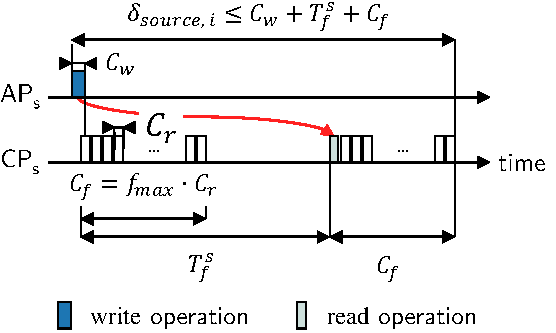
\includegraphics[scale=1]{delta_source_time_graph.pdf}
\caption{Worst-case analysis of the source delay.
\capt{A packet is written as early as possible such that it misses a \opflush and must wait until the next one.}}
\label{fig:delta_source_time_graph}
\end{figure}


%%%%%%%%%%%%%%%%%%%%%%%%%%
%%%%======================
%%%%%%%%%%%%%%%%%%%%%%%%%%


\fakepar{Worst-case analysis of the network delay}
\begin{definition}[Network delay -- $\delta_{network}$]
The network delay is the elapsed time from
a packet being available for communication at the source \cpsrc
until
the end of the communication round where it is served by the wireless protocol (i.e., when it is available at the destination \cpdst).
For a flow \flowi, it is denoted by $\delta_{network, \,i}$.
\end{definition}

\begin{lemma}\label{lem:delta_network}
For any flow \flowi, the network delay is upper-bounded by
\begin{equation}
\label{eq:delta_network}
\delta_{network, \,i} \; \leq \; T_i + D_i + \floor*{\frac{\jitteri + C_f - C_r}{T_f^s}}\cdot T_f^s
\end{equation}
\end{lemma}
\begin{proof}%
As presented in \cref{subsec:details_blink}, \blink guarantees that every packet matching the \emph{expected arrival} is served in a round that terminates before the network deadline $D_i$. Hence, the \emph{delay of an expected packet} is no more than $D_i$.

However, the actual arrival of packets at the source \cpsrc does not match the expected arrival in general, but results from \opflush operations, which occur every $T_f^s$ time unit.
Hence, a packet may arrive \emph{earlier} than the next expected packet. That mismatch between the two arrival times (actual and expected) adds up with the delay of the expected packet (i.e., $D_i$).

Let us consider first that the flow \flowi has no jitter (\ie $\jitteri =0$) and let $m$ be the mismatch between actual and expected arrival time at \cpsrc. $m$ cannot be larger than the flow's minimum message interval $\periodi$
\[
m \;\leq\; \periodi
\]
The intuition is given with \cref{fig:delta_network_time_graph1}. See the caption for details.

\begin{figure}[h!]
\centering
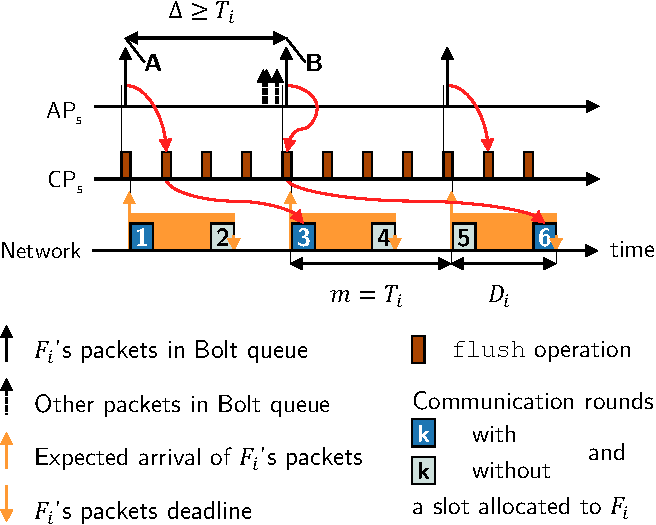
\includegraphics[scale=1]{delta_network_time_graph1.pdf}
\caption{Worst-case analysis of the network delay without jitter.
\capt{Because of the \bolt queue being empty, packet \textbf{A} misses the first flush operation (similarly as in \cref{fig:delta_source_time_graph}), hence the slot allocated to \flowi in round \textbf{1} is wasted. Due to packets released from other flows in the meantime, packet \textbf{B} is flushed directly in the operation preceding round \textbf{3}, in which flow \flowi is allocated a new slot. However, as packet \textbf{A} is still in queue, packet \textbf{B} is not served right away but is delayed until the next allocated slot (\ie in round \textbf{6}). This creates a mismatch of \periodi for packet \textbf{B}.
Furthermore, the mismatch cannot get bigger; assume \textbf{B} were to be available at \cpsrc earlier (\ie one flush operation before, at least), because the time interval between \textbf{A} and \textbf{B} must be at least \periodi, \textbf{A} would arrive earlier as well.
Hence, \textbf{A} would not miss the slot in round \textbf{1}, \textbf{B} would be served in round \textbf{3},
and thus it would yield a smaller mismatch for packet \textbf{B}.}}
\label{fig:delta_network_time_graph1}
\end{figure}


Now, if flow \flowi has also jitter \jitteri, this may entail a bigger mismatch. Actual "arrival" of packets (\ie the epoch when a packet is available for communication at the source \cpsrc, according to the definition of the network delay) can occur only every $T_f^s$ (\ie at the end of one \opflush operation). Therefore, one can see that jitter may induce an extra delay, or mismatch, of roughly $\floor*{\jitteri/T_f^s}\cdot T_f^s$. A more precise analysis of the flushing dynamics (see \cref{fig:delta_network_time_graph2} for details) entails that, overall, the worst-case mismatch $m$ is bounded by

\begin{align}
\label{eq:mismatch}
m \; \leq \;\; &
	T_i + \floor*{\frac{\jitteri + C_f - C_r}{T_f^s}}\cdot T_f^s\\
\intertext{and finally,}
\notag
\delta_{network, \,i} \; \leq \;\; &
	D_i + m \\
\notag
\delta_{network, \,i} \; \leq \;\; &
	T_i + D_i + \floor*{\frac{\jitteri + C_f - C_r}{T_f^s}}\cdot T_f^s \quad \
\end{align}
\end{proof}

\begin{figure}[h!]
\centering
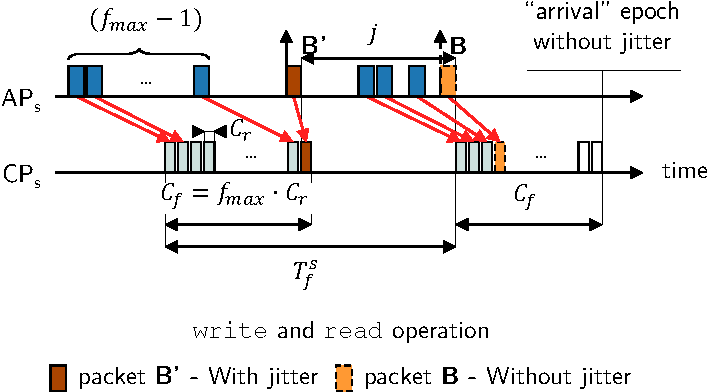
\includegraphics[scale=1]{delta_network_time_graph2.pdf}

\caption{Influence of jitter on the network delay.
\capt{Let us have a closer look at packet \textbf{B} from the previous figure, positioned as early as possible (\ie if it were earlier, so would be \textbf{A}, which would then not miss its slot in round \textbf{1}).
Due to jitter, \textbf{B} is released earlier, say by a amount $j$. This can yield packet \textbf{B'} (\textbf{B} with jitter) to be read out in a previous \opflush operation. In the worst-case, packet \textbf{B'} is read out one operation earlier as soon as $j$ is bigger than $T_f^s - C_f + C_r$, which increases the mismatch $m$ by $T_f^s$. Similarly, $m$ increases by $k \cdot T_f^s$ when $j$ reached  $k \cdot T_f^s - C_f + C_r$, which yields $k = \floor*{\frac{j + C_f - C_r}{T_f^s}}$ and concludes to equation \eqref{eq:mismatch}.
}}
\label{fig:delta_network_time_graph2}
\end{figure}






%%%%%%%%%%%%%%%%%%%%%%%%%%
%%%%======================
%%%%%%%%%%%%%%%%%%%%%%%%%%

\fakepar{Worst-case analysis of the destination delay}

\begin{definition}[Destination delay -- $\delta_{dest}$]
The destination delay is the elapsed time from
a packet being available at the destination \cpdst
until
the end of the \opflush operation where it is read out of \bolt by the destination \apdst (i.e., when it is available for the application).
For a flow \flowi, it is denoted by $\delta_{dest, \,i}$.
\end{definition}


\newpage
\noindent

\begin{lemma}\label{lem:delta_destination}
For any flow \flowi, the destination delay is upper-bounded by
\begin{equation}
\label{eq:delta_destination}
\delta_{dest, \,i} \; \leq \; \nslotsmax*C_w - (\nslotsmax-1)* C_r + T_f^d + C_f
\end{equation}
\end{lemma}

\begin{proof}
The situation is similar as for the source delay, except
that \cpdst writes every $T_{net}$ time unit (\ie after each round) all the packets it received during the last round, which can be as many as \nslotsmax packets.
%\cp writes packets to \bolt sequentially after each communication rounds, where they stay until they are flushed out by AP.
The maximal delay for a packet occurs when it is written too late to be read out during an ongoing \opflush and must wait for the next one.

A careful analysis of the \bolt dynamics shows that the \opread operation is slightly shorter than \opwrite \cite{sutton2015Bolt} (i.e., $C_r < C_w$, see Table \ref{table:simulation_parameters}). Hence, the more packets are written at once by \cpdst, the later a \opflush can start and still miss the last written packet. The worst-case is illustrated on Fig.~\ref{fig:delta_destination_time_graph}. \
\end{proof}

\begin{figure}[h!]
\centering
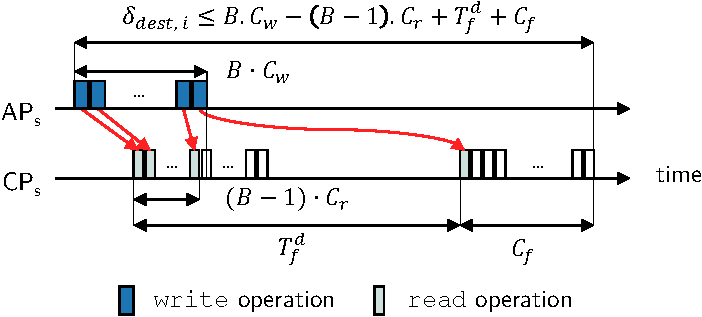
\includegraphics[scale=1]{delta_destination_time_graph.pdf}
\caption{Worst-case analysis of the destination delay.
\capt{A packet is written as early as possible such that it misses a \opflush and must wait until the next one.}}
\label{fig:delta_destination_time_graph}
\end{figure}
